\documentclass[aps,pra,twocolumn,showpacs,superscriptaddress,floatfix,10pt]{revtex4}
\usepackage{graphicx}
\usepackage{psfrag}
\usepackage{amssymb,amsmath}
\usepackage{physics}
\usepackage{float}
\usepackage{dsfont}
\usepackage{algorithmicx}
\usepackage[noend]{algpseudocode}
%\usepackage[dvips]{color}
\algdef{SE}[DOWHILE]{Do}{doWhile}{\algorithmicdo}[1]{\algorithmicwhile\ #1}%

%\setlength{\topmargin}{0.1cm}
\begin{document}
\newcommand{\beq}{\begin{equation}}
\newcommand{\eeq}{\end{equation}}
\newcommand{\ben}{\begin{eqnarray}}
\newcommand{\een}{\end{eqnarray}}
\newcommand{\bea}{\begin{array}}
\newcommand{\eea}{\end{array}}
\newcommand{\om}{(\omega )}
\newcommand{\bef}{\begin{figure}}
\newcommand{\eef}{\end{figure}}
\newcommand{\leg}[1]{\caption{\protect\rm{\protect\footnotesize{#1}}}}
\newcommand{\ew}[1]{\langle{#1}\rangle}
\newcommand{\be}[1]{\mid\!{#1}\!\mid}
\newcommand{\no}{\nonumber}
\newcommand{\etal}{{\em et~al }}
\newcommand{\geff}{g_{\mbox{\it{\scriptsize{eff}}}}}
\newcommand{\da}[1]{{#1}^\dagger}
\newcommand{\cf}{{\it cf.\/}\ }
\newcommand{\ie}{{\it i.e.\/}\ }   

\newcommand{\spazio}{\vspace{0.3cm}}%{\vspace{1.05cm}}
\hyphenation{bio-mol-ecules}
\newcommand{\de}[1]{\frac{\partial}{\partial{#1}}}
\newcommand{\U}{\tilde{U}}
\newcommand{\V}{\tilde{V}}


\title{Improved State Discrimination of Optical Quantum Ensembles through the use of Ancillas}

\author{Jake~A.~Smith}
\affiliation{Tulane University, Department of Physics, New Orleans, Louisiana 70118, USA}

\author{Lev Kaplan}
\affiliation{Tulane University, Department of Physics, New Orleans, Louisiana 70118, USA}

 \begin{abstract}
 	Finish the experiment first before writing abstract.
\end{abstract}                                                               
\date{\today}
\pacs{***}
\maketitle

\section{Basic Mathematical Principles}
\label{Intro}
An optical quantum state of $N$ photons contained in $M$ optical modes can be written in the Fock basis,
\begin{eqnarray}
	\label{LO State Fock Basis}
	\ket{\psi} = c_1 \ket{N,0,\dots,0_M} + c_2 \ket{N-1,1,0,\dots, 0_M} + \\* \dots  + c_{d_H} \ket{0,0,\dots,N_M}	\nonumber \quad \quad \quad \quad
\end{eqnarray}
We note that the Hilbert space dimension of such a state is given by
\begin{equation}
\label{Hilbert Space Dimension}
	d_H = \frac{(N+M-1)!}{N!(M-1)!}
\end{equation}
or the number of ways to order $N$ indistinguishable photons and $M-1$ partitions.

A linear optical operation acting on such a state is generally described by the transformation of creation operators:
\begin{equation}
\label{LO Creation Operator Transformation}
\hat{a}^\dagger_\alpha \rightarrow \sum_{\beta=1}^{M} U_{\alpha\beta} \hat{a}^\dagger_\beta
\end{equation}
where $U_{\alpha \beta}$ are the elements of some unitary complex matrix, $U$. Thus, one typically converts a state in the form of~(\ref{LO State Fock Basis}) into
\begin{eqnarray}
\ket{\psi} = \Big(c_1 \frac{(\hat{a}^\dagger_1)^N}{\sqrt{N!}} + c_2 \frac{ (\hat{a}^\dagger_1)^{N-1} \hat{a}^\dagger_2}{\sqrt{(N-1)!}} + \dots \\* + c_{d_H} \frac{(\hat{a}^\dagger_M)^N}{\sqrt{N!}}\Big) \ket{0,0,\dots,0_M} \quad \quad \nonumber
\end{eqnarray}
and applies the symbolic transformation~(\ref{LO Creation Operator Transformation}). This may be fine for an optical circuit of few components and small $N$ and $M$, but transforming the creation operators for large systems can otherwise become intractable. Instead, we use a numerical protocol to simulate this process, which we will discuss briefly in the following section.

Before we begin, we can define $A(U)$ as the complex matrix which represents the action of~(\ref{LO Creation Operator Transformation}) on a quantum state in the Fock basis~(\ref{LO State Fock Basis}). The output state of an optical circuit $\ket{\psi^\prime}$ will determined by standard matrix-vector multiplication
\begin{equation}
\label{Matrix Vector Product}
\ket{\psi^\prime} = A(U) \ket{\psi}
\end{equation}
The matrix elements $U_{\alpha \beta}$ in~(\ref{LO Creation Operator Transformation}) are assumed to be the very same as those of $U$ in $A(U)$. If $N \ge 2$, the group of all linear optical operators, $ A(U) \in \textbf{A}$, is a proper (strict) subgroup of the general unitary group
\begin{equation}
\label{Proper Subgroup}
\textbf{A} \subset \textbf{GU}(d_H).
\end{equation}
Thus, not all quantum logic operations on Fock states can be implemented via linear optical circuits.
\section{Simulating Linear Optical State Evolution}
\label{Section of Facts}
For an optical circuit of $K$ number of components,
\begin{equation}
	\label{Fact 1}
A(U_K) A(U_{K-1}) \dots A(U_1) = A(U_1 U_2 \dots U_K)
\end{equation}
Each component $U_k$ could be a simple beam splitter, phase shifter, or a general integrated circuit consisting of many low-level components.
(\ref{Fact 1}) allows us to simulate the net effect of a series of low-level linear optical operations with efficiency. We can compile the $K$ optical hardware components via the matrix multiplication $U_1 U_2 \dots U_K$, rather than evolve the state in a series of discrete steps.

Rewriting~(\ref{LO State Fock Basis}) as
\begin{equation}
\label{LO State Fock Vec Basis}
\ket{\psi} = \sum_{\vec{n}} c_{\vec{n}} \ket{\vec{n}}
\end{equation}
where
\begin{equation}
\ket{\vec{n}} = \ket{n_1,n_2,\dots,n_M}
\end{equation}
are the Fock states, we define
\begin{equation}
\label{m definition}
\ket{\vec{m}(\vec{n})} = \ket{m_1,m_2,\dots,m_N}
\end{equation}
as \textit{any} vector where $m_\alpha$ is the mode-location of photon number $\alpha$. There can be many vectors $\ket{\vec{m}(\vec{n})}$ for each $\ket{\vec{n}}$, since photons are generally indistinguishable and labeling them is an arbitrary process. We simply need to choose \textit{some} labeling and pick any valid $\ket{\vec{m}(\vec{n})}$. Then the elements of $A(U)$ are given by
\begin{eqnarray}
\label{Fact 2}
A(U)_{\vec{n}^\prime,\vec{n}} = \quad \quad \quad \quad \quad \quad \quad \quad \quad \quad \quad \quad \quad \quad \quad \quad \quad \\ \small \nonumber \prod_{p=1}^{M} \frac{\sqrt{n_p^\prime !}}{\sqrt{n_p !}} \left[\sum_{perm(\vec{m}^\prime)} U_{m_1 m_1^\prime} U_{m_2 m_2^\prime} \dots U_{m_N m_N^\prime} \right] \outerproduct{\vec{n}^\prime}{\vec{n}} 
\end{eqnarray}
where the summation is over all distinct permutations of integer entries in the vector $\vec{m}^\prime$. A more complete discussion of the numerical methods used here and proof of Eq.~\ref{Fact 1}-\ref{Fact 2} are available in~\cite{Jake Smith}.
\section{The Classical Mutual Entropy}
The purpose of our work here is to improve quantum state discrimination at the receiving end of a quantum communication channel. As a gauge for the success of the quantum measurement, we choose the classical mutual entropy $H(X:Y)$ which is defined as the amount of overlapping information encoded by the sender, Alice, and extracted by the receiver, Bob;
\begin{equation}
H(X:Y) = \sum_{x \in X} \sum_{y \in Y} p(x,y) \log_2 \frac{p(x,y)}{p(x) p(y)}
\end{equation}
where $X$ is the encoding variable and $Y$ is the decoding variable.
We can tailor this definition of the mutual information to better suit our needs. First, we can isolate the Shannon information of Alice's classical encoding, $H(X)$,
\begin{eqnarray}
\small H(X:Y) = \sum_{x,y} p(x,y) \log_2 \frac{p(x,y)}{p(y)} \\
- \sum_{x,y} p(x,y) \log_2 p(x) 
\end{eqnarray}
and apply the law of total probability
\begin{eqnarray}
& -\sum_{x,y} p(x,y) \log_2 p(x) = -\sum_x \log_2 p(x) \sum_y p(x,y) \nonumber \\ & = -\sum_x p(x) \log_2 p(x)
\end{eqnarray}
Defining the classical Shannon entropy
\begin{equation}
\label{Shannon Entropy}
	H(X) = -\sum_{x \in X} p(x) \log_2 p(x)
\end{equation}
leaves us with
\begin{equation}
\label{Mutual Entropy Full}
\small
	H(X:Y) = H(X) - \sum_{\substack{x \in X \\ y \in Y}} p(x) p(y|x) \log_2 \frac{\sum_{x^\prime} p(x^\prime) p(y|x^\prime)}{p(x) p(y|x)}.
\end{equation}
To maximize the communication efficiency of a quantum channel, we can numerically maximize Eq.~\ref{Mutual Entropy Full}.
For any ensemble where all $p(x) = 1/\abs{X}$, we can simplify the mutual entropy further,
\begin{equation}
\label{Mutual Entropy}
H(X:Y) = \log_2 \abs{X} - \frac{1}{\abs{X}} \sum_{x,y} p(y|x) \log_2 \frac{\sum_{x^\prime} p(y|x^\prime)}{p(y|x)}
\end{equation}
The conditional entropy
\begin{equation}
\label{Conditional Entropy}
\small H(X|Y) =  \frac{1}{\abs{X}} \sum_{\substack{x \in X \\ y \in Y}} p(y|x) \log_2 \frac{\sum_{x^\prime \in X} p(y|x^\prime)}{p(y|x)}
\end{equation}
is sufficient to quantify the success of a quantum measurement in this case. 

The Holevo bound~\cite{Holevo,Jake Smith}
\begin{equation}
	H(X:Y) \le S(\rho) \le H(X)
\end{equation}
tells us that the mutual information shared between Alice and Bob is limited by the von Neumann entropy of the encoded states,
\begin{equation}
	S(\rho) = - \tr( \rho \log_2 \rho )
\end{equation}
We'll refer to this quantity as the channel encoding capacity.

\section{Discrimination of the Bell States Encoded in the Dual Rail}
Previous work in maximizing the encoding capacity of an optical quantum channel~\cite{First Paper} revealed that imposing a \textit{linear optical} encoding (Alice uses only linear optical operations to encode information into a quantum ensemble) does not prevent her from achieving the true channel capacity. But any relationship counselor will tell you that real communication generally requires a good listener; just because Alice was able to optimally compress information into the channel, does not guarantee Bob will be able to extract it. In fact, we typically observe that Bob is not able to fully discriminate an a-priori set of optical quantum states if he is restricted to a linear optical photo-counting von Neumann measurement. Formally, we define our encoded ensemble of quantum states
\begin{equation}
\{\ket{\psi_1},\ket{\psi_2},...\ket{\psi_{\abs{X}}}\},
\end{equation}  
each sent over the channel with probability $p_x$
and photo-counting measurement operators
\begin{equation}
\{ \outerproduct{\vec{n}_1}{\vec{n}_1}, \outerproduct{\vec{n}_2}{\vec{n}_2}, \dots , \outerproduct{\vec{n}_{\abs{Y}}}{\vec{n}_{\abs{Y}} } \}.
\end{equation}
A photo-counting von Neumann measurement is defined here as a unitary linear optical transformation followed by a photo-counting measurement. The probability of measuring outcome $y$ assuming state $x$ was sent will be
\begin{eqnarray}
\label{von Neumann conditional probability part 1}
\ket{\psi_x^\prime} = A(U) \ket{\psi_x} \\
\label{von Neumann conditional probability part 2}
p(y|x) = \abs{\braket{\vec{n}_y}{\psi_x^\prime}}^2.
\end{eqnarray}
Imposing this measurement scheme, the Holevo bound appears to become strict for any optical communication channel
\begin{equation}
	H(X:Y) < S(\rho).
\end{equation}
Closing the Holevo bound here is prevented by two completely separate issues. First, $\rho$ may consist of a set of non-orthogonal states. Perfectly distinguishing a set of non-orthogonal states is a general problem in quantum mechanics and a number of solutions have been proposed~\cite{Hausladen,Lloyd,Lloyd Other,Ogawa,Nagaoka,Hayashi}. Second, we are often unable to construct, even for an ensemble of orthogonal states, the necessary linear optical operator $A(U)$ to rotate all states into  non-overlapping subspaces. Here, we will focus exclusively on this second problem and attempt to improve state discrimination of a set of orthogonal quantum states. In particular, we examine the Bell states encoded in the dual-rail, defined as
\begin{eqnarray}
\rho  = \sum_{i=1}^4 \frac{1}{4} \outerproduct{\psi_i}{\psi_i} \quad \quad \quad \quad \quad \\
\ket{\psi_1} = \frac{1}{\sqrt{2}} \ket{1,0,1,0} + \frac{1}{\sqrt{2}} \ket{0,1,0,1} \\
\ket{\psi_2} = \frac{1}{\sqrt{2}} \ket{1,0,1,0} - \frac{1}{\sqrt{2}} \ket{0,1,0,1} \\
\ket{\psi_3} = \frac{1}{\sqrt{2}} \ket{1,0,0,1} + \frac{1}{\sqrt{2}} \ket{0,1,1,0} \\
\ket{\psi_4} = \frac{1}{\sqrt{2}} \ket{1,0,0,1} - \frac{1}{\sqrt{2}} \ket{0,1,1,0}
\end{eqnarray}
For this ensemble, $S(\rho)$ and $H(X)$ are both fixed at 2 bits. Numerical minimization of Eq.~(\ref{Conditional Entropy}) with Eq.~(\ref{von Neumann conditional probability part 1}) and Eq.~(\ref{von Neumann conditional probability part 2}) suggests that the optimal von Neumann measurement one can apply to this system will extract $H(X:Y) = 1.5$ bits. This is accomplished by first applying the operator $A(U)$ where
\begin{equation}
\label{First U}
U = \frac{1}{2} \begin{pmatrix} 1 & 1 & 1 & 1 \\ 1 & -1 & 1 & -1 \\ 1 & -1 & -1 & 1 \\ 1 & 1 & -1 & -1 \end{pmatrix}   
\end{equation}
and then performing a photon-counting measurement. Thus, the Bell states encoded in the dual rail form a simple, symmetric, quantum ensemble in which full state discrimination is not immediately possible. 
\section{Augmenting the System with Ancilla Resources}
\label{Augmenting Section}
Previous work in linear optical quantum computing suggests that supplementing a system with ancilla photons and modes is known to improve control over a quantum state. In particular, the gate fidelity of a measurement-assisted CNOT~\cite{KLM} acting on qubits encoded in the dual-rail improves dramatically with the proper use of ancilla resources \cite{Uskov}. So we expect to see some benefit to incorporating ancilla states here, and that is indeed the case. Our numerical experiments consisted of minimizing Eq.~(\ref{Conditional Entropy}) with Eq.~(\ref{von Neumann conditional probability part 2}) but instead of using Eq.~(\ref{von Neumann conditional probability part 1}) to define $\ket{\psi_x^\prime}$, we set
\begin{equation}
\label{Matrix Vector Product Ancilla}
\ket{\psi_x^\prime} = A(U) \ket{\psi_a} \otimes \ket{\psi_x}.
\end{equation}
In  Fig.~(\ref{Decoding Hardware Ancillas}) we present an illustration of the decoding apparatus described by Eq~(\ref{Matrix Vector Product Ancilla}). The ancilla state is defined as any Fock state constructed from $N_a$ ancilla photons and $M_a$ ancilla modes 
\begin{eqnarray}
& \ket{\psi_a} = c_1 \ket{N_a,0,\dots,0_{M_a}} + c_2 \ket{N_a-1,1,0,\dots, 0_{M_a}} + \nonumber \\ & \dots  + c_{d_{H_a}} \ket{0,0,\dots,(N_a)_{M_a}}	 \quad \quad \quad \quad
\end{eqnarray}
\begin{equation}
d_{H_a} = \frac{(N_a+M_a-1)!}{N_a ! (M_a-1)!}
\end{equation}
Because we allow photons to freely cross the boundary between computational and ancilla modes under the application of $A(U)$, the tensor product in Eq.~(\ref{Matrix Vector Product Ancilla}) falls strictly within the larger physical Hilbert space. In other words, $A(U)$ is not a square matrix. In Table~\ref{Ancilla Resources Table} we present results of numerical optimization over the unitary operator, $U$ and ancilla state $\ket{\psi_a}$.
\begin{figure}[ht]
	\centering
	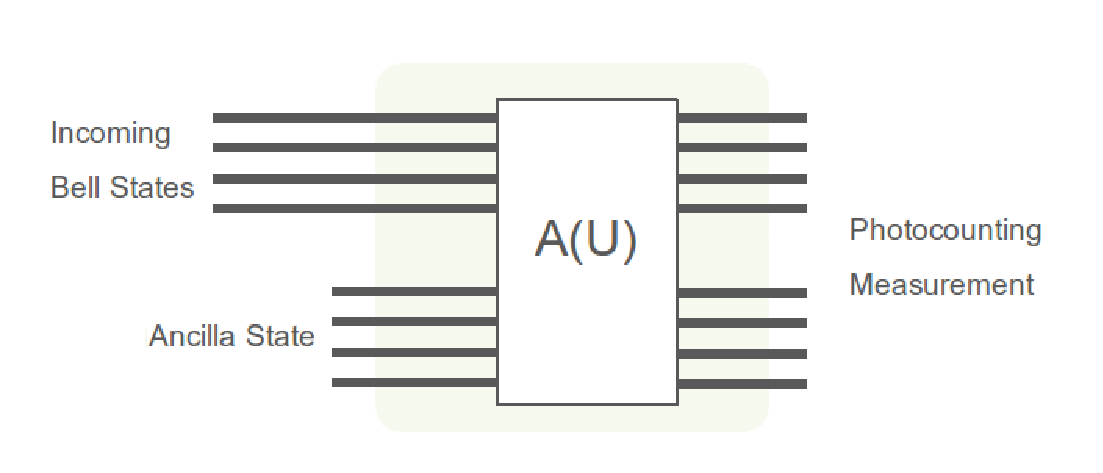
\includegraphics[width= 0.5 \textwidth]{./ancillaMeasApp.pdf}
	\caption{At the receiving end of a linear optical quantum channel, we build this measurement apparatus. Bell states arrive in the top four optical modes and we have a simple ancilla state prepared in the bottom set of modes. A linear optical transformation is applied, and then a photocounting measurement is performed.}
	\label{Decoding Hardware Ancillas}
\end{figure}
\begin {table}[H]
\begin{center}
	\begin{tabular}{l*{6}{c}r} 
		& & & &  $M_a$ \\
		&       & \vline   & 0 & 1 & 2 & 3 & 4 \\
		\cline{2-8}
		&	0    & \vline  & 1.5 & 1.5 & 1.5 & 1.5 & 1.5 \\
		&      1    & \vline & - & 1.5 & 1.5 & 1.5 & 1.5 \\
		$N_a$ & 2 & \vline & - & 1.5 & 1.625 & 1.625 & 1.625 \\
		& 3 & \vline & - & 1.5 & 1.625 & 1.625 & 1.625 \\
		& 4 & \vline & - & 1.5 & 1.625 & 1.625 & 1.75 \\
	\end{tabular}
	\caption{Results for maximization of $H(X:Y)$ in bits over the operator $A(U)$ and states $\ket{\psi_a}$ for ancilla photons $N_a$ and ancilla modes $M_a$. In a perfect measurement, $H(X:Y) \rightarrow 2$ bits.\label{Ancilla Resources Table}}
\end{center}
\end{table}
Table~\ref{Ancilla Resources Table} reports a discrete improvement in state discrimination with each additional pair of ancilla resources. We observe that all solutions converge to ancilla states $\ket{\psi_a}$ in a simple, classical state;
\begin{equation}
\ket{\psi_a} \equiv \ket{1,1,\dots,1_{M_a}}
\end{equation} In particular we present results for $N_a,M_a=0$, $N_a,M_a=2$ and $N_a, M_a= 4$. Each of these solutions represents a family of solutions which are equivalent under symmetry (e.g. invariant permutations of columns since the labeling of output modes is arbitrary). 
\newline


		$ H(X:Y) = 1.5 $ bits
		$$ \ket{\psi_a} = \ket{NULL} $$
		\begin{equation}
		\label{No Ancillas}
		U = \frac{1}{2} \begin{pmatrix} 1 & 1 & 1 & 1 \\ 1 & -1 & 1 & -1 \\ 1 & -1 & -1 & 1 \\ 1 & 1 & -1 & -1 \end{pmatrix}   
		\end{equation}
		$$or$$
		\begin{equation}
		U = \frac{1}{\sqrt 2} \begin{pmatrix} 1 & 1 & 0 & 0 \\ 0 & 0 & 1 & 1 \\ 1 & -1 & 0 & 0 \\ 0 & 0 & 1 & -1 \end{pmatrix}   
		\end{equation}

		$ H(X:Y) = 1.625 $ bits
		$$ \ket{\psi_a} = \ket{1,1} $$
		\begin{equation}
		\label{11 Ancilla}
		U = \frac{1}{2} \begin{pmatrix} 
		1 & 1 & 1 & 1 & 0 & 0 \\ 
		1 & -1 & 1 & -1 & 0 & 0 \\ 
		\frac{1}{\sqrt 2} & \frac{-1}{\sqrt 2} & \frac{-1}{\sqrt 2} & \frac{1}{\sqrt 2} & 1 & 1 \\ 
		\frac{1}{\sqrt 2} & \frac{1}{\sqrt 2} & \frac{-1}{\sqrt 2} & \frac{-1}{\sqrt 2} & i & -i \\
		\frac{1}{\sqrt 2} & \frac{1}{\sqrt 2} & \frac{-1}{\sqrt 2} & \frac{-1}{\sqrt 2} & -i & i \\
		\frac{1}{\sqrt 2} & \frac{-1}{\sqrt 2} & \frac{-1}{\sqrt 2} & \frac{1}{\sqrt 2} & -1 & -1 \\
		\end{pmatrix}   
		\end{equation}
		$$or$$
		\begin{equation}
		U = \frac{1}{2} \begin{pmatrix} 
		1 & 1 & 1 & 1 & 0 & 0 \\ 
		1 & -1 & 1 & -1 & 0 & 0 \\ 
		\frac{1}{\sqrt 2} & \frac{-1}{\sqrt 2} & \frac{-1}{\sqrt 2} & \frac{1}{\sqrt 2} & \sqrt 2 & 0 \\ 
		\frac{1}{\sqrt 2} & \frac{1}{\sqrt 2} & \frac{-1}{\sqrt 2} & \frac{-1}{\sqrt 2} & 0 & -i \sqrt 2 \\
		\frac{1}{\sqrt 2} & \frac{-1}{\sqrt 2} & \frac{-1}{\sqrt 2} & \frac{1}{\sqrt 2} & -\sqrt 2 & 0 \\
		\frac{1}{\sqrt 2} & \frac{1}{\sqrt 2} & \frac{-1}{\sqrt 2} & \frac{-1}{\sqrt 2} & 0 & i \sqrt 2 \\
		\end{pmatrix}   
		\end{equation}
		$$or$$
		\begin{equation}
		U = \frac{1}{2} \begin{pmatrix} 
		1 & 1 & 1 & 1 & 0 & 0 \\ 
		1 & -1 & 1 & -1 & 0 & 0 \\ 
		1 & 0 & -1 & 0 & 1 & 1 \\
		0 & 1 & 0 & -1 & -1 & 1 \\
		1 & 0 & -1 & 0 & -1 & -1 \\
		0 & 1 & 0 & -1 & 1 & -1 
		\end{pmatrix}   
		\end{equation}
		$ H(X:Y) = 1.75 $ bits
		\newline
		$$ \ket{\psi_a} = \ket{1,1,1,1} $$
		\newline
		\begin{equation}
		\label{1111 Ancilla}
		U = \frac{1}{2} \begin{pmatrix} 
		1 & 1 & 1 & 1 & 0 & 0 & 0 & 0 \\ 
		1 & -1 & 1 & -1 & 0 & 0 & 0 & 0 \\ 
		0 & 0 & 0 & 0 & 1 & 1 & 1 & 1 \\
		0 & 0 & 0 & 0 & 1 & -1 & 1 & -1 \\
		\frac{1}{\sqrt 2} & \frac{1}{\sqrt 2} & \frac{-1}{\sqrt 2} & \frac{-1}{\sqrt 2} & \frac{1}{\sqrt 2} & \frac{1}{\sqrt 2} & \frac{-1}{\sqrt 2} & \frac{-1}{\sqrt 2} \\ 
		\frac{1}{\sqrt 2} & \frac{-1}{\sqrt 2} & \frac{-1}{\sqrt 2} & \frac{1}{\sqrt 2} & \frac{1}{\sqrt 2} & \frac{-1}{\sqrt 2} & \frac{-1}{\sqrt 2} & \frac{1}{\sqrt 2} \\ 
		\frac{1}{\sqrt 2} & \frac{1}{\sqrt 2} & \frac{-1}{\sqrt 2} & \frac{-1}{\sqrt 2} & \frac{-1}{\sqrt 2} & \frac{-1}{\sqrt 2} & \frac{1}{\sqrt 2} & \frac{1}{\sqrt 2} \\ 
		\frac{1}{\sqrt 2} & \frac{-1}{\sqrt 2} & \frac{-1}{\sqrt 2} & \frac{1}{\sqrt 2} & \frac{-1}{\sqrt 2} & \frac{1}{\sqrt 2} & \frac{1}{\sqrt 2} & \frac{-1}{\sqrt 2} \\ 
		\end{pmatrix}   
		\end{equation}
Restating our definition of a linear optical transformation
\begin{equation}
\hat{a}^\dagger_i \rightarrow \sum_j U_{i j} \hat{a}_j^\dagger
\end{equation}
and noting that all ancilla modes are ordered \textit{before} computational modes, our results seem to suggest a general trend of spreading each pair of additional ancilla modes over four of the output modes, with discrete phase differences of $\pi$. Extrapolating these solutions, one could guess
\begin{eqnarray}
&N_a = 6, M_a = 8 : \quad \ket{\psi_a} = \ket{1,1,1,1,1,1,0,0} \nonumber \\ & \quad H(X:Y) \rightarrow 1.875 \mbox{ bits} \nonumber
\end{eqnarray}
since the three pairs of ancilla photons would then have room to spread over 12 output modes. One could further extrapolate
\begin{eqnarray}
& N_a = 8, M_a = 12 : \quad \ket{\psi_a} = \ket{1,1,1,1,1,1,1,1,0,0,0,0} \nonumber \\  & \quad H(X:Y) \rightarrow 2.0 \mbox{ bits} \nonumber
\end{eqnarray}
since the four pairs of ancilla photons have room to spread over 16 output modes. 
\newline
\newline
Unfortunately, while Eq.~(\ref{Fact 2}) allows for feasible numerical simulation of these physical systems, the large optimization space and overwhelming saturation of local minima within it prevent us from reaching a global solution. Minimization methods including BFGS, conjugate gradient descent, Levenberg-Marquardt, Nelder-Meade, and principal axis were all tried with no success. In addition, we optimized over non-unitary operators in the place of $U$ which was also unsuccessful. Pushing to simulations of this size, we recommend trying a method other than numerical optimization to find an optimal $U$.
\section{Global Quantum Channel Optimization}
In Section~\ref{Augmenting Section} we discussed using ancilla resources to improve the discrimination of states in a quantum ensemble at the receiving end of a linear optical quantum channel. We found that ancilla resources can help us to control and decode multi-photon states, though we were unable to find a protocol for perfect measurement.  Here, we finally attempt to optimize the \textit{total} capacity of a linear optical quantum channel using ancillas in the decoding phase. We allow Alice to perform a non-orthogonal encoding and we allow Bob to perform a von Neumann measurement with the help of ancilla resources, as in Fig.~\ref{Decoding Hardware Ancillas}. The full communication protocol is defined as follows;
\newline
\begin{center}
	\begin{minipage}{20em}
		(1) An entangled initial state, $\ket{\psi_1}$ is pre-distributed between Alice and Bob.
		\newline
		\newline
		(2) Alice performs some operation, $A(U_x)$ with probability $p(x)$ where $U_1 = I$ and $U_2,U_3, \dots, U_{\abs{X}}$ are unitary matrices operating only on her modes.
		\newline
		\newline
		(3) Alice's modes run to Bob, who now has possession of the entire state.
		\newline
		\newline
		(4) Bob augments the system with some pre-generated ancilla state $\ket{\psi_a}$, applies an operation to all modes $A(U_B)$, and performs a photocounting measurement.
	\end{minipage}
\end{center}
~
\newline
An illustration of the full device is presented in Fig.~(\ref{Total Quantum Channel Device}).
Formally, we want to perform a projective measurement on the ensemble of states;
\begin{equation}
\rho = \sum_{x \in X}  p(x) \outerproduct{\psi_x^\prime}{\psi_x^\prime}
\end{equation}
\begin{equation}
\ket{\psi_x^\prime} = A(U_B) A(U_x) \ket{\psi_1} \otimes \ket{\psi_a}.
\end{equation}
where according to Eq.~(\ref{Fact 1}),
\begin{equation}
A(U_B) A(U_x) = A(U_x U_B).
\end{equation}
\begin{figure}[ht]
	\centering
	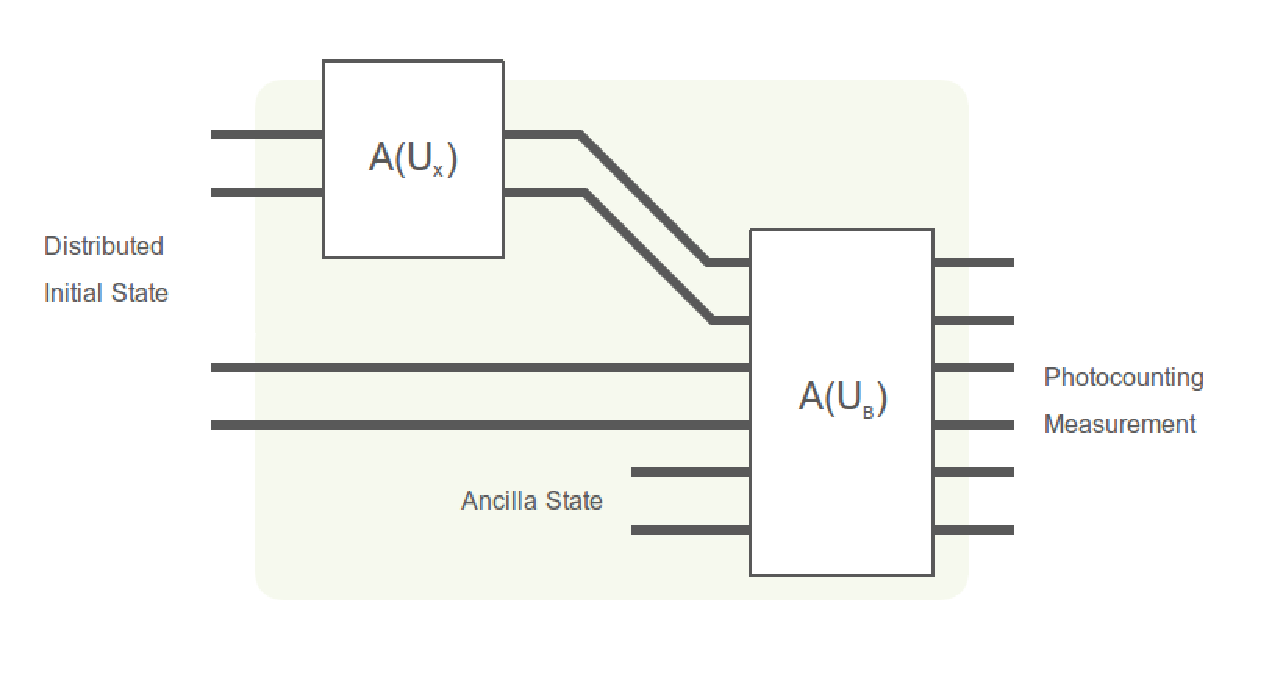
\includegraphics[width= 0.5 \textwidth]{./GlobalApparatus.pdf}
	\caption{Schematic for the total communication device. Alice and Bob each initially possess two modes. Alice acts on her modes with some operation $A(U_x)$ : $x \in X$. Alice's modes run to Bob, who augments the system with some ancilla state over two modes, applies the operation $A(U_B)$ and does a photocounting measurement.}
	\label{Total Quantum Channel Device}
\end{figure}
\newline
To quantify the success of Bob's photocounting measurement we use the mutual entropy as defined in Eq.~(\ref{Mutual Entropy Full}) and 
\begin{equation}
p(y|x) = \abs{\braket{\vec{n}_y}{\psi_x^\prime}}^2.
\end{equation}
Revisiting the key physical devices in~\cite{First Paper}, we incrementally increase the number of encoding symbols $\abs{X}$ and maximize the mutual entropy $H(X:Y)$. We then augment the systems with ancillas and attempt to close the Holevo bound. The reader should take note of our potentially confusing notation; $N_A$ and $M_A$ refer to the number of photons and modes initially in Alice's possession. $N_a$ and $M_a$ refer to the number of ancilla photons and modes that Bob augments to incoming states.
\subsection{$N=2,M=4,M_A=2$}
This system was of special interest in~\cite{First Paper} because Alice was able to achieve a maximum encoding by building an orthogonal ensemble of quantum states. We recall that in this case
\begin{eqnarray}
\abs{X} = 8 \quad \quad \quad \quad  \\
S(\rho)_{max} = \log_2 d_S = \log_2 8 = 3 \mbox{ bits}
\end{eqnarray}
\section{Conclusion}
We'll see.
\acknowledgments
I want to thank my moms, yo. This research was supported in part using high performance computing (HPC) resources and services provided by Technology Services at Tulane University, New Orleans, LA.
\begin{thebibliography}{99}

\bibitem{Jake Smith} (meeee) Other paper we're working on

\bibitem{Holevo} A. S. Holevo, Probl. Peredachi Inf. \textbf{9}, 110 (1973).	

\bibitem{First Paper} J. A. Smith, D.B. Uskov, L. Kaplan Phys. Rev. A \textbf{92}, 022324 (2015).

\bibitem{KLM}  E. Knill, R. Laflamme, G. J. Milburn, Nature (London) 409, 46 (2001).

\bibitem{Uskov} Uskov Et. Al.
Phys. Rev. A 79, 042326 (2009).

\bibitem{Adami} https://arxiv.org/abs/quant-ph/9806048

\bibitem{Review Paper} Kok Et. Al.
Rev. Mod. Phys. 79, 135 (2007).

\bibitem{Hausladen} P. Hausladen, R. Jozsa, B. Schumacher, M. Westmoreland, and W. K. Wootters, Phys. Rev. A. \textbf{54}, 1869, (1996).

\bibitem{Lloyd} S. Lloyd, V. Giovannetti, and L. Maccone, Phys. Rev. Lett. \textbf{106}, 250501 (2011).

\bibitem{Lloyd Other} V. Giovannetti, S. Lloyd, and L. Maccone, Phys. Rev. A \textbf{85}, 012302, (2012).


\bibitem{Ogawa} T. Ogawa, IEEE Trans. Inf. Theory \textbf{45}, 2486 (1999).

\bibitem{Nagaoka} T. Ogawa and H. Nagaoka, IEEE Trans. Inf. Theory \textbf{53}, 2261 (2007).

\bibitem{Hayashi} M. Hayashi and H. Nagaoka, IEEE Trans. Inf. Theory \textbf{49}, 1753 (2003).

\end{thebibliography}


\end{document}
